\newpage
\subsection{Students Page}
The students page is divided into three sections: “dashboard”, “Subjects” and “Request for Course”. The main area of the dashboard section contains the total number of enrolled courses details. By clicking to the “view” button under each course the details and materials about the course is shown.\\

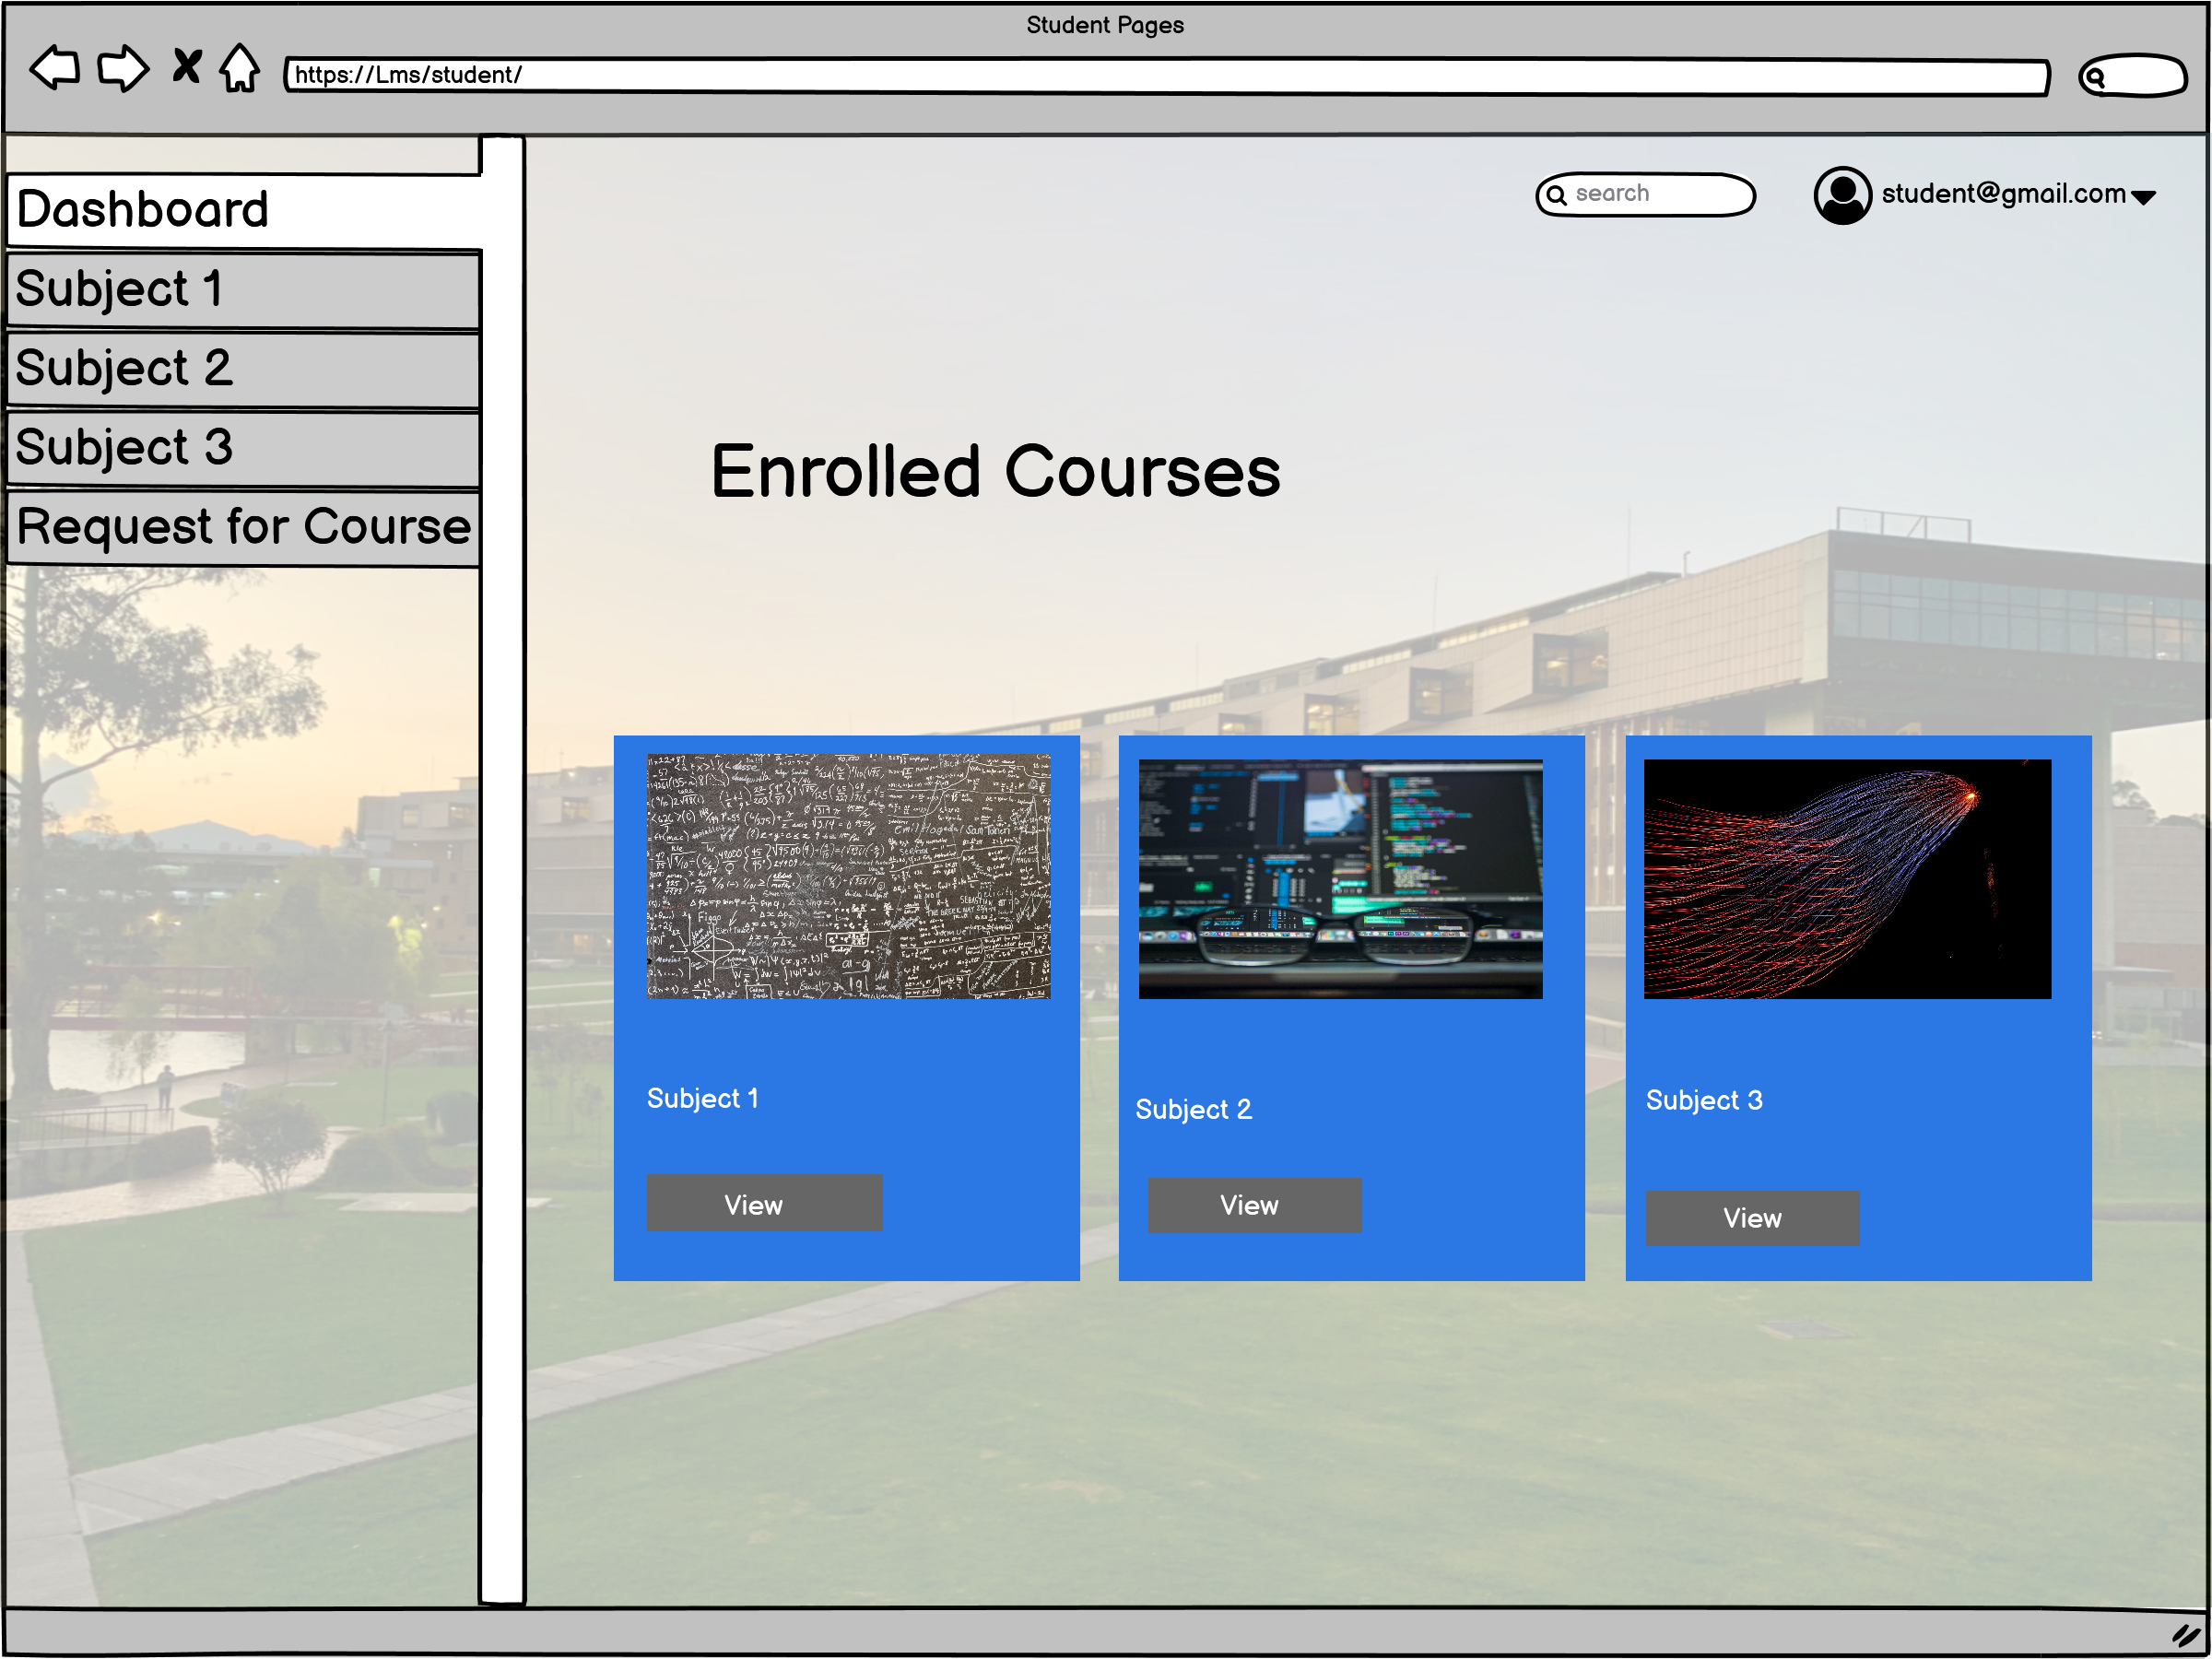
\includegraphics[width=\columnwidth]{images/Student Form.png}
\newpage
On the subjects page there are the material folder introducing all the information about particular course with dates and necessary links.\\

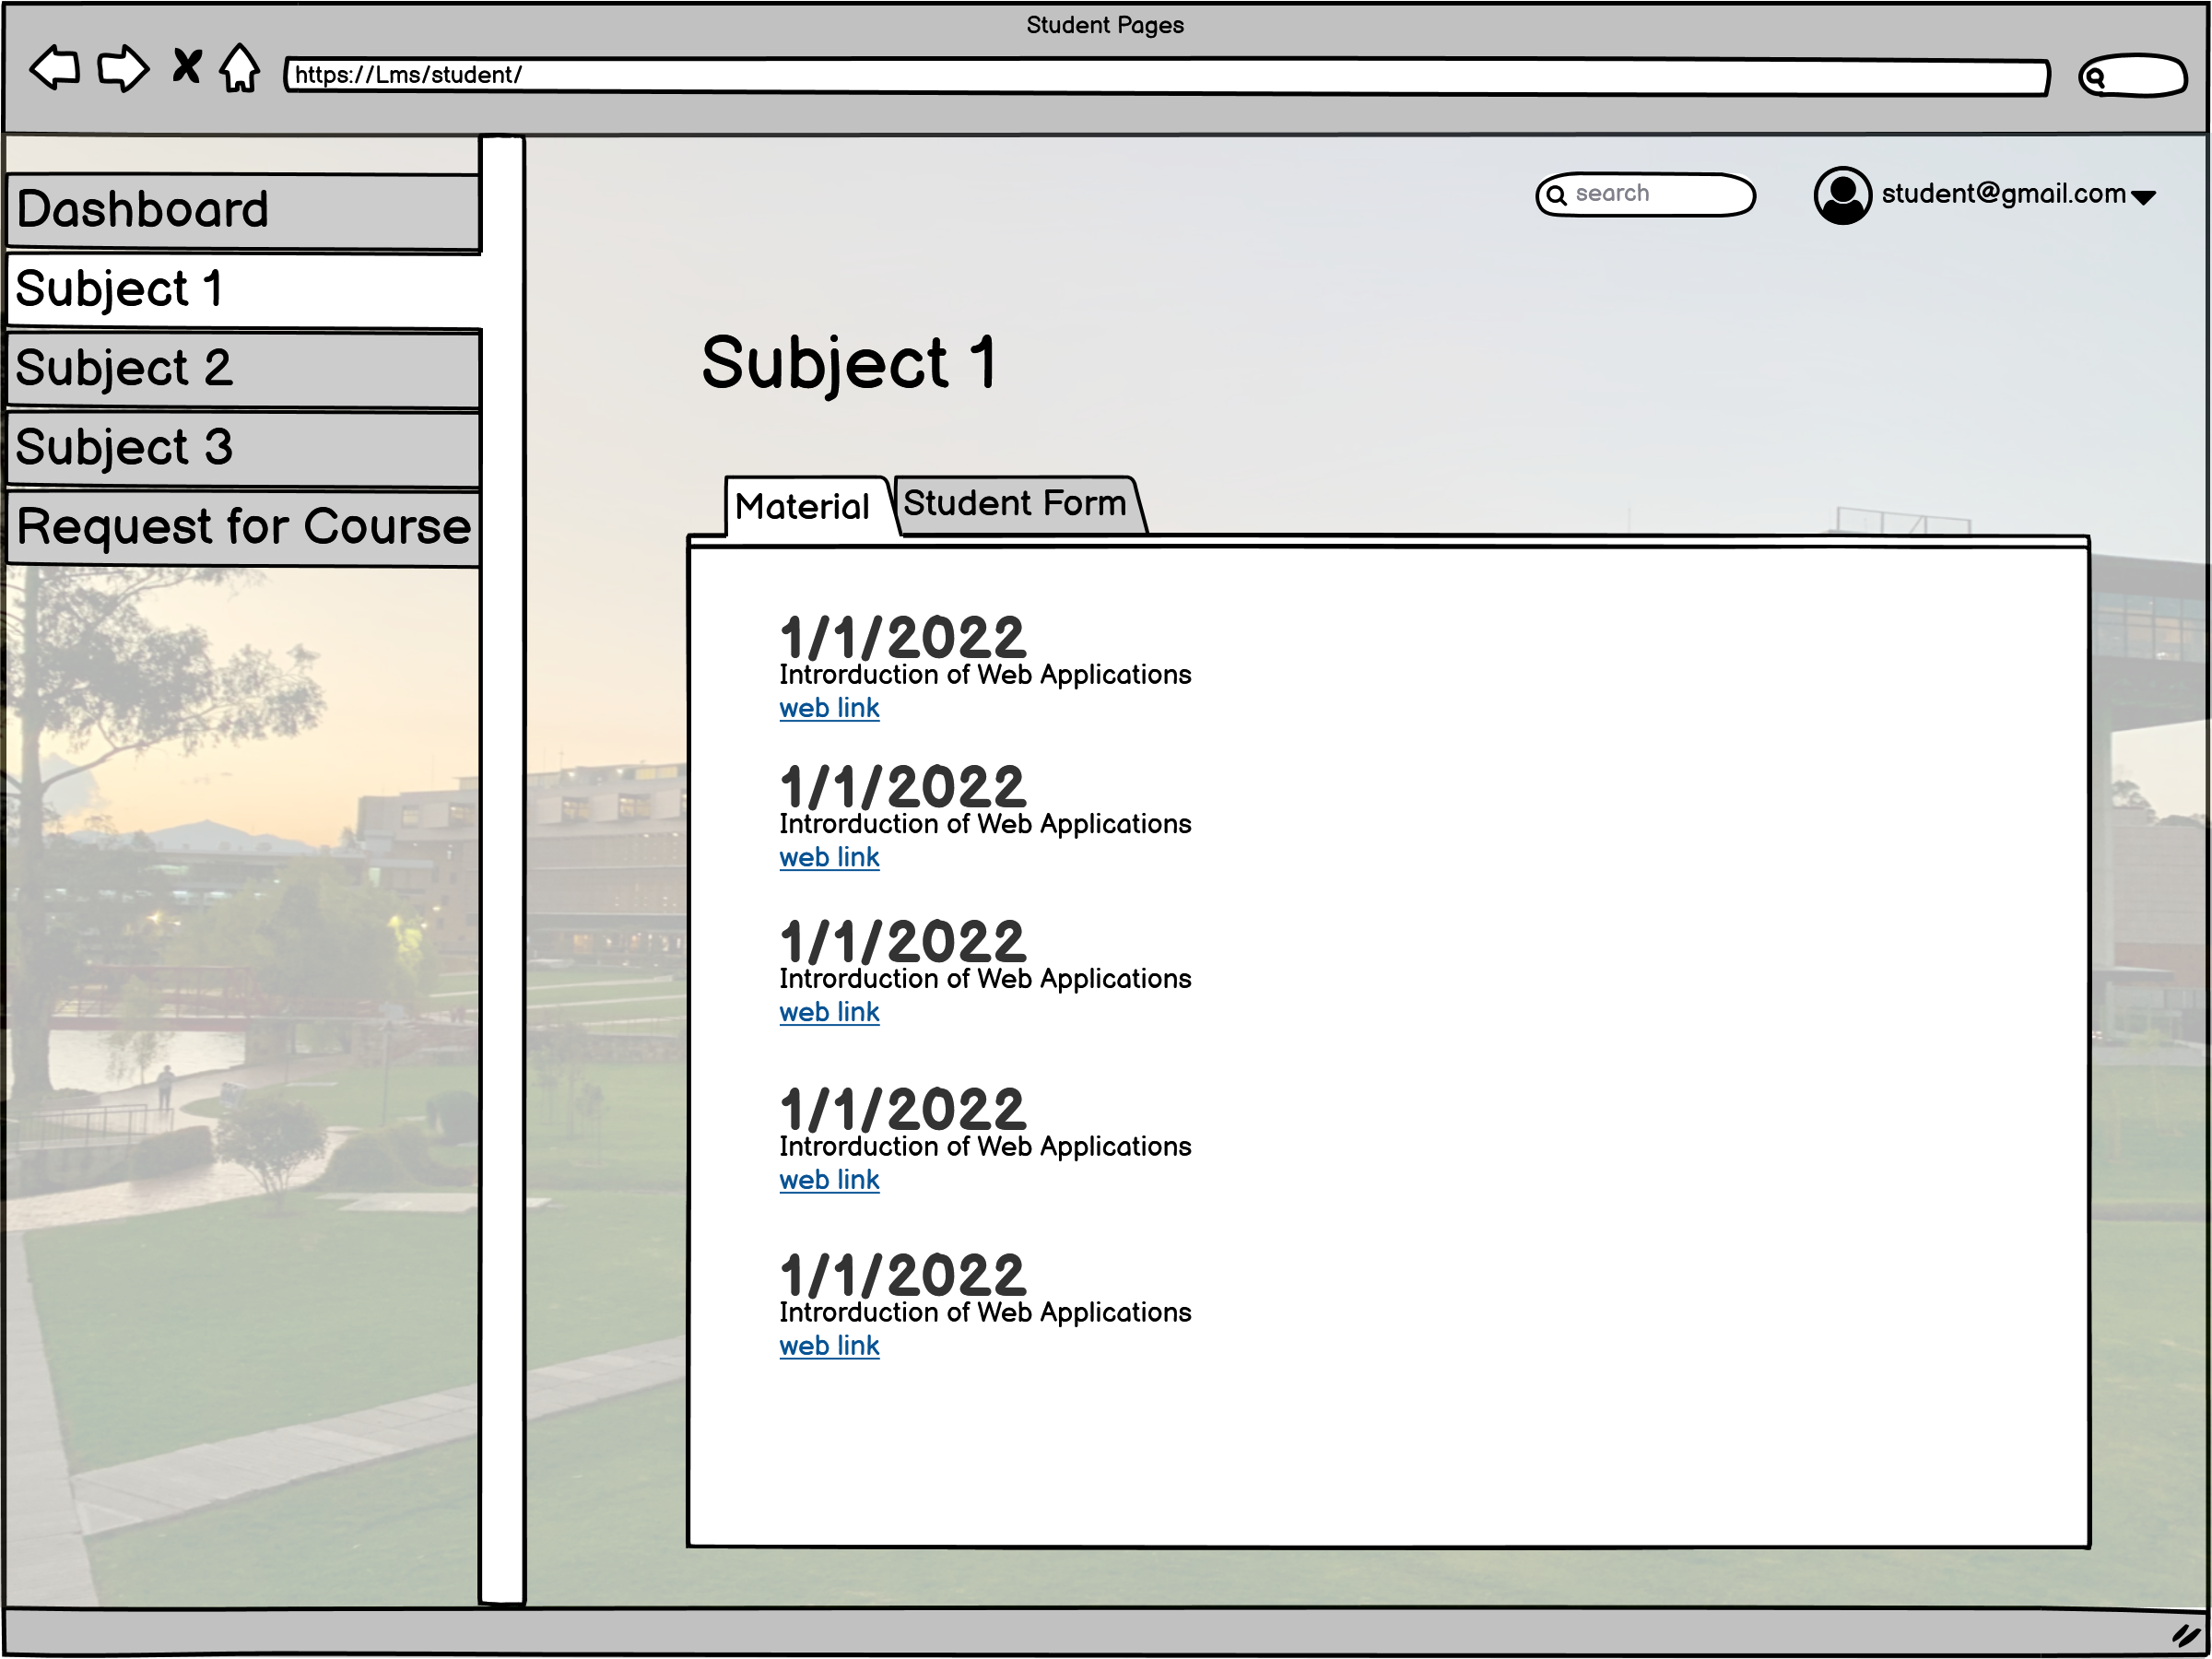
\includegraphics[width=\columnwidth]{images/Subject 1 student.png}\\

Clicking to the “Student Form” folder there is a form for filling in manually by the student. The topic and the description of the message should be written and send by clicking the “send” button.\\

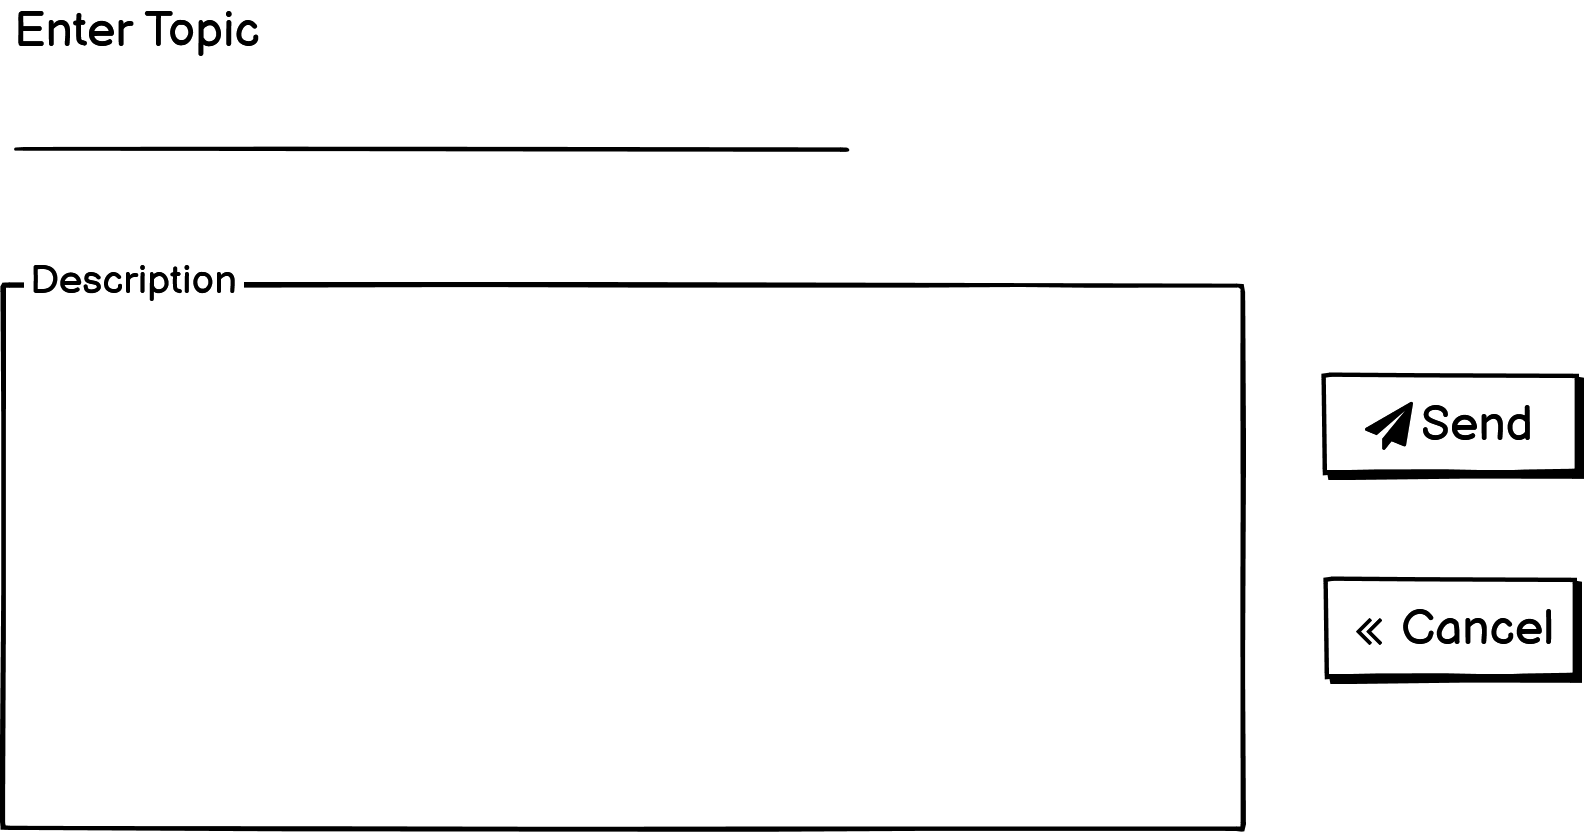
\includegraphics[width=0.65\columnwidth]{images/Student Form_2.png}
\newpage
The Request for course part is for sending the request in order to enroll to the course. There are the “select” button for choosing the course the student want to be enrolled in and the chosen course description prerequisite.\\

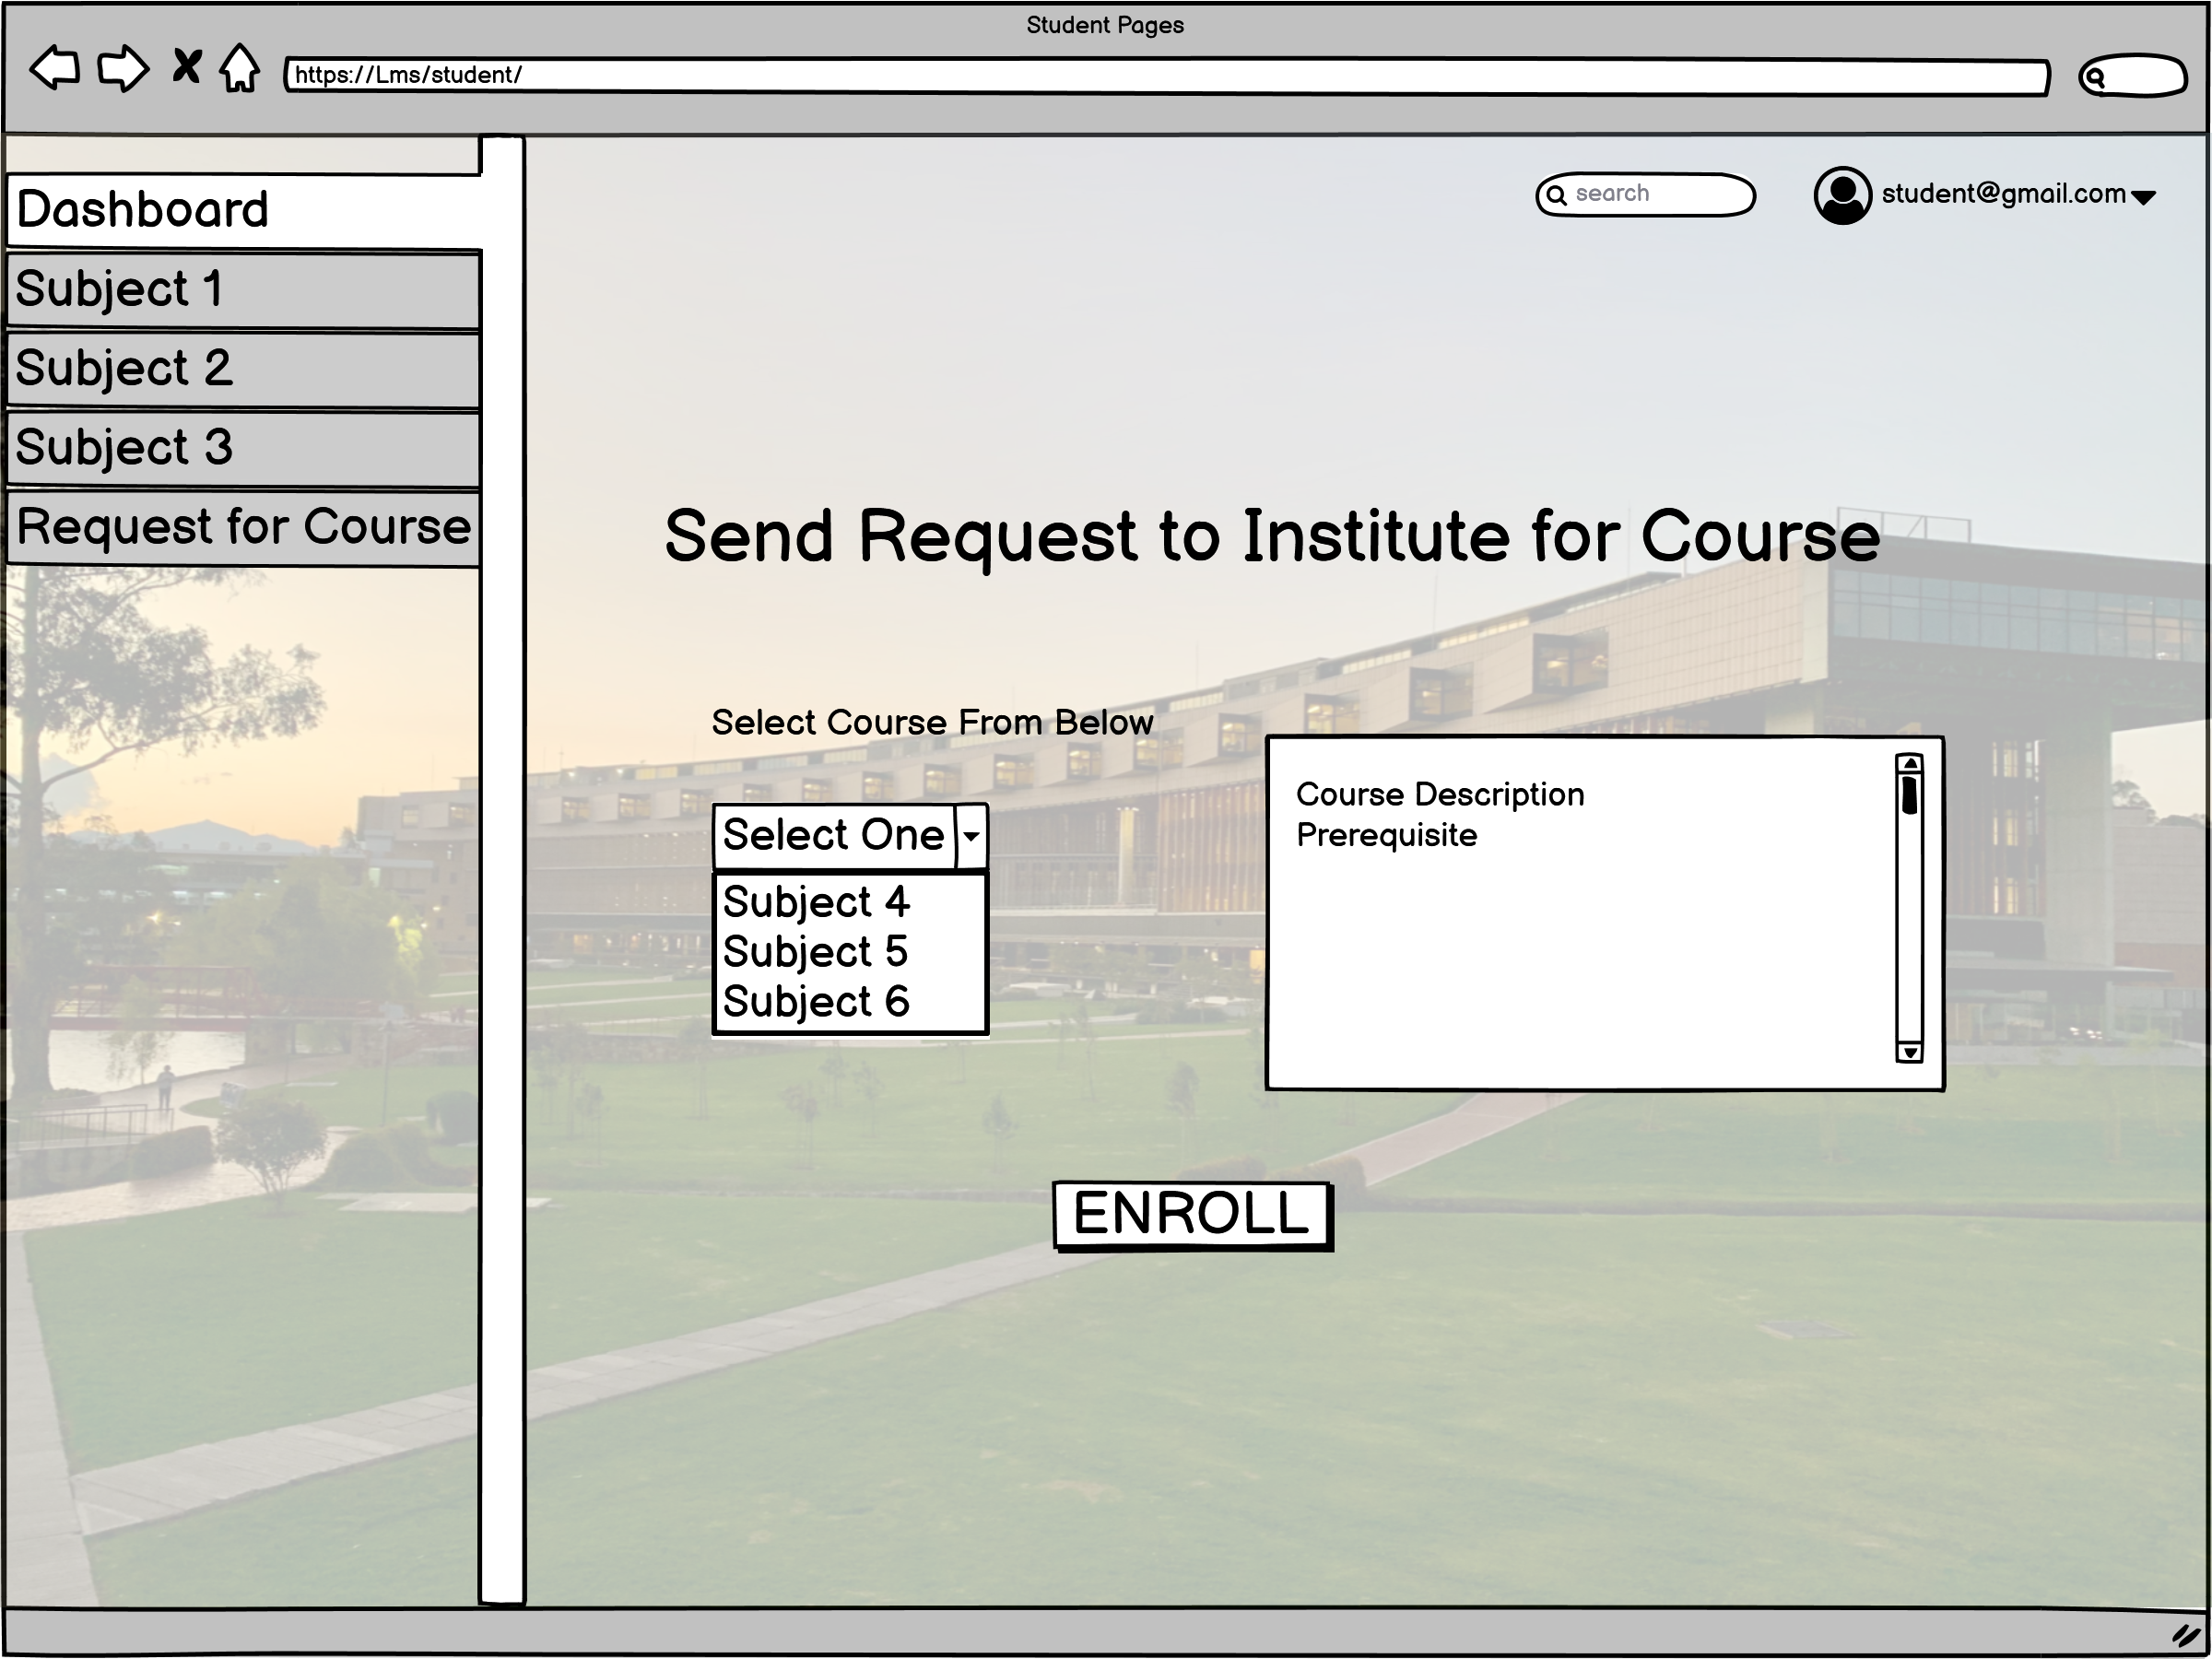
\includegraphics[width=\columnwidth]{images/Request for Course.png}